\documentclass[11pt]{article}
\usepackage[margin=1in, top=1in]{geometry}
\usepackage[all]{nowidow}
\usepackage[hyperfigures=true, hidelinks, pdfhighlight=/N]{hyperref}
\usepackage[separate-uncertainty=true, group-digits=true]{siunitx}
\usepackage{graphicx,amsmath,physics,tabto,float,amssymb,pgfplots,verbatim,tcolorbox}
\usepackage{listings,xcolor,subfig,caption,import,wrapfig,enumitem}
\usepackage[version=4]{mhchem}
\usepackage[noabbrev]{cleveref}
\newcommand{\creflastconjunction}{, and\nobreakspace}
\definecolor{stringcolor}{HTML}{C792EA}
\definecolor{codeblue}{HTML}{2162DB}
\definecolor{commentcolor}{HTML}{4A6E46}
\captionsetup{font=small, belowskip=0pt}
\lstdefinestyle{appendix}{
    basicstyle=\ttfamily\footnotesize,commentstyle=\color{commentcolor},keywordstyle=\color{codeblue},
    stringstyle=\color{stringcolor},showstringspaces=false,numbers=left,upquote=true,captionpos=t,
    abovecaptionskip=12pt,belowcaptionskip=12pt,language=Python,breaklines=true,frame=single}
\lstdefinestyle{inline}{
    basicstyle=\ttfamily\footnotesize,commentstyle=\color{commentcolor},keywordstyle=\color{codeblue},
    stringstyle=\color{stringcolor},showstringspaces=false,numbers=left,upquote=true,frame=tb,
    captionpos=b,language=Python}
\renewcommand{\lstlistingname}{Appendix}
\pgfplotsset{compat=1.17}

\begin{document}

\begin{center}
    \textbf{CP Test 1}\hspace{1.5in}\textbf{KDSMIL001}\hspace{1.5in}\textbf{14-05-2022}
\end{center}
\rule{\textwidth}{1pt}

\begin{enumerate}
    \item \begin{enumerate}
        \item We begin, when integrating using Gauss-Laguerre quadrature, by transforming the integrals in question,
        \begin{equation}
            I = \frac{\int_0^\infty (x^4 +1)xe^{-\sqrt{4x^2 +1}}dx}{\int_0^\infty xe^{-\sqrt{4x^2 +1}}dx}
            \label{eqn:Q1Integral}
        \end{equation}
        into ones of the form
        \begin{equation}
            \int_0^\infty f(x)e^{-x}.
            \label{eqn:GaussLaguerreGenForm}
        \end{equation}
        We begin with the numerator, which we will call $I_N$. Choosing the substitution $w=\sqrt{4x^2+1}$, we get
        \begin{equation*}
            x=\sqrt{\frac{w^2-1}{4}}, \;\;\; x^4+1=\left(\frac{w^2-1}{4}\right)^2+1, \;\;\; dx=\frac{w}{2\sqrt{w^2-1}}dw 
        \end{equation*}
        Then we find 
        \begin{align*}
            I_N&=\int_1^\infty \frac{w}{2\sqrt{w^2-1}} \left(\left(\frac{w^2-1}{4}\right)^2+1\right) \sqrt{\frac{w^2-1}{4}} e^{-w} dw\\
            &=\int_0^\infty \frac{w}{4}\left(\left(\frac{w^2-1}{4}\right)^2+1\right)e^{-w} dw
        \end{align*}
        Using another substitution, $x=w-1$, we can see 
        \begin{equation}
            I_N = \int_0^\infty \frac{x+1}{4}\left(\left(\frac{x^2+2x}{4}\right)^2+1\right)e^{-x-1}
            \label{eqn:q1iNumerator}
        \end{equation}
        where we easily identify
        \begin{equation}
            f_N(x) = \frac{x+1}{4e}\left(\left(\frac{x^2+2x}{4}\right)^2+1\right).
            \label{eqn:q1iFN}
        \end{equation}
        For the denominator, we use the same two substitutions, finding
        \begin{align}
            I_D &= \int_0^\infty xe^{-\sqrt{4x^2 +1}}dx \nonumber\\
            &=\int_1^\infty \frac{w}{4}e^{-w} dw \nonumber\\
            &=\int_0^\infty \frac{x+1}{4e}e^{-x} dx \label{eqn:q1iDenominator}\\
            \implies f_D(x) &= \frac{x+1}{4e}. \label{eqn:q1iFD}
        \end{align}
        We can then use Gauss-Laguerre quadrature to find these integrals:
        \begin{align}
            I_N &\approx \sum_{i=1}^n f_N(x_i)w_i \label{eqn:GLNumerator}\\
            I_D &\approx \sum_{i=1}^n f_D(x_i)w_i \label{eqn:GLDenominator}
        \end{align}
        where the $x_i$ are the roots of the $n$-th order Laguerre polynomial, and $w_i$ are the respective weights. These can be found using \texttt{np.polynomial.laguerre.laggauss(n)}.\\
        Using a 16-th order Laguerre polynomial, we found $I \approx 10.250000000000082$, which is pretty bang on $10.25$.

        \item For a Monte Carlo integration method, we choose the Metropolis method, as the integral in \cref{eqn:Q1Integral} is of the form
        \begin{equation}
            I = \frac{\int p(x)f(x)dx}{\int p(x)dx}.
            \label{eqn:MetropolisGeneralForm}
        \end{equation}
        We can identify $f(x)=x^4+1$, and thus we need to sample according to 
        \begin{equation}
            p(x) = xe^{-\sqrt{4x^2 +1}}.
            \label{eqn:q1iiProbDist}
        \end{equation}
        Using the Metropolis method allows us to not have to normalise this $p(x)$, which is nice as the integral of it is a bit ugly.\\
        To begin with, we generate $N_0=\num[]{500000}$ points $x_i$, according to $p(x)$ using the Metropolis random walk/Markov chain method. In order to avoid correlation between points we compute the autocorrelation function 
        \begin{equation}
            C(j) = \frac{\langle x_{i+j}x_i\rangle - \langle x_i \rangle^2}{\langle x_i^2 \rangle - \langle x_i \rangle^2}
            \label{eqn:Autocorrelation}
        \end{equation}
        for a range of $j$ values, and find the first $j$ for which $C(j)\leq 0.01$. \Cref{fig:correlation} shows the results.

        \begin{figure}[h]
            \begin{center}
                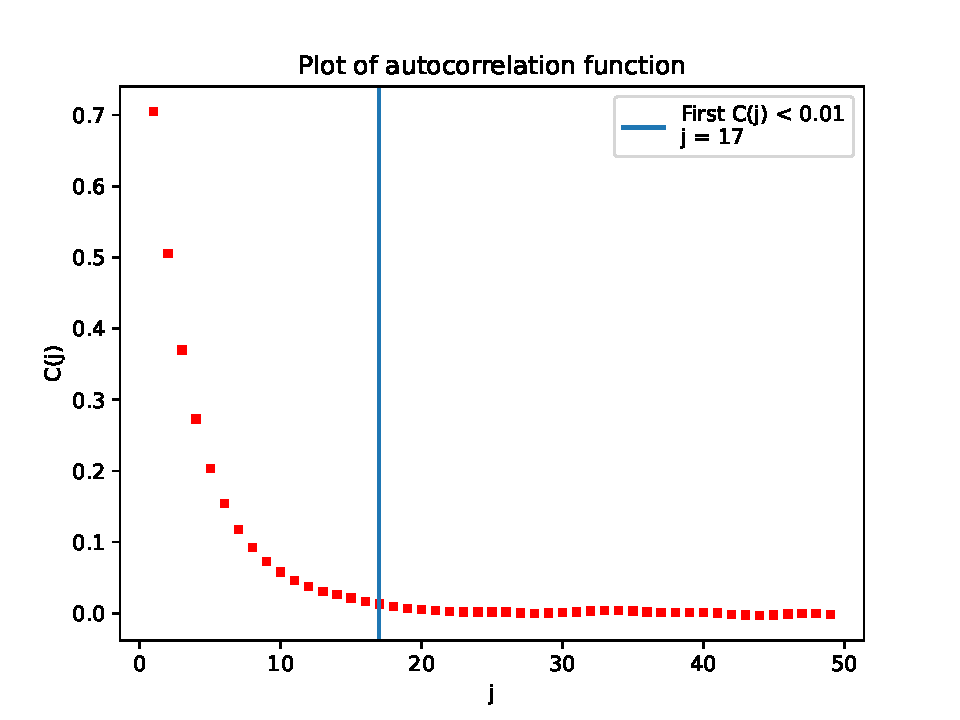
\includegraphics[width=.75\textwidth]{Plots/correlation.pdf}
                \caption{Plot of the autocorrelation function for the $N_0$ generated values, giving us $C(j=17)$ as the first value $\leq 0.01$. }
                \label{fig:correlation}
            \end{center}
        \end{figure}

        This tells us how many numbers in the Markov chain to skip each time we choose one to be part of our final distribution. We also need to consider the starting values, as the method goes through a transient phase before equilibrating. To find how many numbers to chop off the start, we can find the moving average of the $N_0$ generated values, and see when it begins to level level off. \Cref{fig:equilibrium} shows the results.

        \begin{figure}[h]
            \begin{center}
                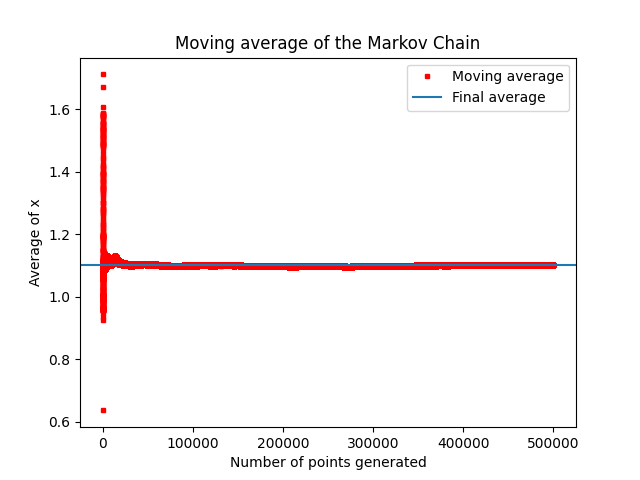
\includegraphics[width=.75\textwidth]{Plots/equilibrium.png}
                \caption{Plot of the moving average of the $N_0$ points in the generated Markov chain, along with the final average, to see when the moving average begins to level off.}
                \label{fig:equilibrium}
            \end{center}
        \end{figure}
        
        By inspection, we can see it levels off at around \num[]{20000} points, so we choose to cut off the first \num[]{20000} points. Doing this and skipping every 17 points leaves us with around \num[]{28000} points in our distribution. \Cref{fig:histogram} shows the results. 
        
        \begin{figure}[h]
            \begin{center}
                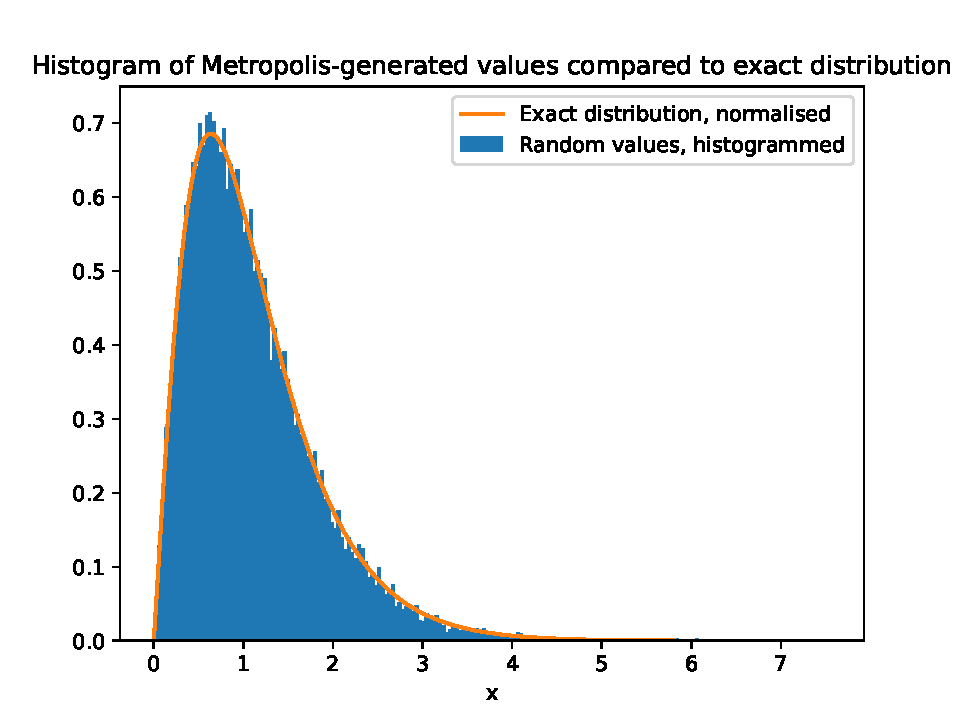
\includegraphics[width=.6\textwidth]{Plots/histogram.pdf}
                \caption{Histogram of the $x$-values calculated using the Metropolis method, distributed according to \cref{eqn:q1iiProbDist}, along with the exact distribution. Note that the histogram is normalised to 1 over the interval shown, while $p(x)$ is normalised over the semi-infinite interval, so there may be some discrepancies.}
                \label{fig:histogram}
            \end{center}
        \end{figure}
        
        With these randomly generated numbers $x_i$, we can finally compute $I$ in \cref{eqn:Q1Integral} using
        \begin{equation}
            I \approx \frac{1}{N}\sum_{i=1}^N f(x_i)
            \label{eqn:}
        \end{equation}
        

    \end{enumerate}
    


\end{enumerate}
% I = 10.479278962481828 +/- 0.29186577473165193
\end{document}